% $Id$

\chapter{Multiple Kernel Learning example}
\label{data_example3}
\minitoc


This chapter will describe the steps necessary to perform a classification with SimpleMKL \url{http://asi.insa-rouen.fr/enseignants/~arakoto/code/mklindex.html} \cite{Rakotomamonjy2008} using PRoNTo. These are similar to the ones in Chapter \ref{sec:Block_design_fMRI_dataset}, thus, the reader is advised to complete the tutorial in Chapter \ref{sec:Block_design_fMRI_dataset}  before moving on, since the explanation of some steps will be less detailed.

Many practical learning problems involve multiple and heterogeneous data sources. In this way, Multiple Kernel Learning (MKL) \cite{Bach2004} has been proposed to combined different data sources in a single predictive model by learning the relative contribution of each kernel (often corresponding to each data source) to the model. In MKL, the kernel $K$  can  be  considered  as  a  linear  combination  of $M$ `basis kernels'. For further details, please refer to \cite{Bach2004}.

One example of a MKL approach based on SVM is the SimpleMKL algorithm \cite{Rakotomamonjy2008}. Essentially, the algorithm is based on a gradient descent on the SVM objective value and iteratively determine the combination of kernels by a gradient descent wrapping \cite{Rakotomamonjy2008}. For further details, please refer to \cite{Rakotomamonjy2008}

We will use the same dataset used in Chapter \ref{sec:Block_design_fMRI_dataset}, this fMRI dataset originates from a study on face and object representation in human ventral temporal cortex \cite{Haxby2001}. The dataset\footnote{Pre-processed (realigned and normalised) data from participant 1.} used in this chapter can be found in PRoNTo's website \url{http://www.mlnl.cs.ucl.ac.uk/pronto/prtdata.html} (data set 1) and the whole\footnote{Not pre-processed.} dataset is available in \url{http://data.pymvpa.org/datasets/haxby2001/}.

For simplicity, in this example we will use PRoNTo to predict if the subject is viewing an image of a Face or a House based on the fMRI scans. We will classify the whole brain images using SimpleMKL and a leave one block out cross-validation scheme.

\section{GUI analysis}

We will first analyse the data using PRoNTo's GUI and then repeat the analysis using the {\tt matlabbatch} system.

To start, create a new directory in which to save the results of the analysis, then start up \matlab{} and type `prt' or `pronto' in the \matlab{} prompt. This will open the main interface of PRoNTo.

%--------------------------------------------------------------------------

\subsection{Data \& Design}


\begin{itemize}
	
	\item In PRoNTo's main window, click on `Data \& Design'. Like in the previous chapters, browse the directory in which to save the PRT structure (saved as `PRT.mat');
	
	\item In the panel `Groups', click on `Add' and provide a name to the group (we only have one group/subject), with no spaces, e.g. `G1';
	
	\item Add a subject in the `Subject/Samples' option, e.g. `S1', and leave the `Samples' tick box below the panel unchecked. See Chapter \ref{chap:DataDesign} of the manual for more information on this option;
	
	\item In the `Modalities' panel, click on `Add' and provide a name to the modality, e.g. `fMRI'. In the `Data format', choose `nifti'. In the `Design' field, choose the option `Load SPM.mat'. This file is available with the Haxby dataset on PRoNTo's website\footnote{http://www.mlnl.cs.ucl.ac.uk/pronto/prtdata.html} inside the folder Haxby\_dataset/design/. Finally, in this case leave `Regression targets' as it is, in the `No targets' option.
	

	\begin{itemize}
		
		\item The reader is referred to Chapter \ref{sec:Block_design_fMRI_dataset} and chapter \ref{chap:DataDesign} for the case where there is no `SPM.mat' file available.
	
	\end{itemize}
	
	
	\item Finally, load all the image files available in the fMRI directory (Haxby\_dataset/fMRI/). You can select all the files by using the right mouse button and clicking on the option `Select All'. When all the images are selected, click on the `Done' button;
	
	\item In the `Masks' field, on the bottom left of the `Data and design' window, select the `whole\_brain' mask for the specified modality. The mask is available in the masks directory inside the folder Haxby\_dataset/masks/;

	\item Click on the `Review' button to check the data and the design inserted for this modality. For more information on what one can do with the Review option, please see Chapter \ref{chap:DataDesign};
	
	\item Click on the `Save' button to create the `PRT.mat' file with the structure containing the information that has been previously specified. If no errors are shown in the \matlab{} command, leave the `Data and design' window by clicking `Quit'. The `Data and design' window should look similar to the one in Figure \ref{fig:gui_data_and_designs_final} from the previous chapter.
	
\end{itemize}

%--------------------------------------------------------

\subsection{Prepare feature set}

\begin{itemize}
	
	\item Next we have to prepare the feature set, so click on `Prepare feature set' in PRoNTo's main window. A new window will open prompting you to select a PRT.mat file. Select the `PRT.mat' file previously created in the `Data \& Design' step, as in Figure \ref{fig:gui_prepare_featureSet_choose_PRT} from Chapter \ref{sec:Block_design_fMRI_dataset}. Once you click `Done' another window will appear, `Specify modality to include', as in Figure \ref{fig:gui_prepare_featureSet_specify_modality} from Chapter \ref{sec:Block_design_fMRI_dataset}. Here you set the specification of different parameters and options for each modality, which are:
	
	\begin{itemize}
		\item `Modality' field: select the modality previously specified in the `Data \& Design' step, `fMRI';
		\item `Conditions' field: select `All scans';
		\item `Parameters' box: select the polynomial detrend with order 1 and the 'No scaling' option;
		\item `Features' box: select the `Build one kernel per region' tick box and load the `AAL' atlas (named 'aal\_79x91x69') available in the PRoNTo directory (PRoNTo/atlas/). Then, click on the 'Done' button. The final `Specify modality to include' window should look similar to the one in Figure \ref{fig:data_example3_gui_prepare_featureSet_specify_modality};
		
			
		\begin{figure}[!h]
	\centering
		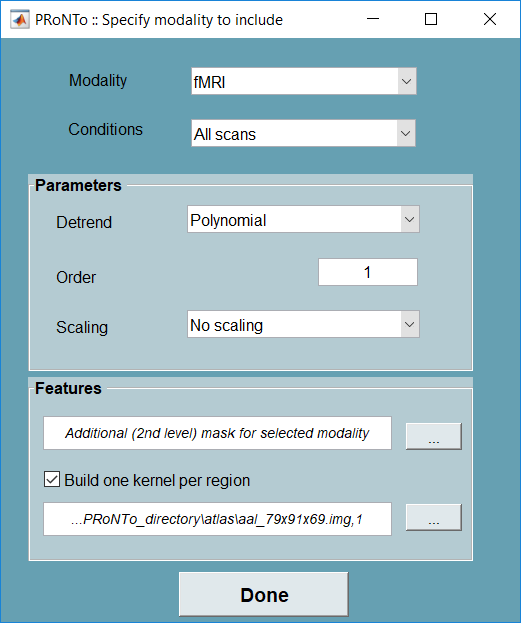
\includegraphics[scale=0.6]{images/Tutorial/v3/data_example3/data_example3_gui_prepare_featureSet_specify_modality.png}
	\caption{`Specify modality to include' GUI final configuration.}
	\label{fig:data_example3_gui_prepare_featureSet_specify_modality}
\end{figure}	
		
			%\begin{itemize}
			%\item As an optional step, in the `Additional mask for selected modality' field, the user can specify a `second-level' mask, which can be used to select regions of interest (ROIs) in which the classification can be performed. For instance, we can enter the `fusiform\_gyrus' mask available with this dataset; 
			%\end{itemize}	
			
		
	\end{itemize}		
		
		\item Once you specify the modality to include and click `Done', yet another window will appear, `Prepare feature set'. Here you provide a name for the feature set, e.g. `HaxbyFeatures' and finally you click on `Build kernel / data matrix' to build the kernel. If everything was done correctly, a progress bar will pop up, marking the start of the procedure, similar to the Figure \ref{fig:gui_prepare_featureSet_prepare_and_build} from Chapter \ref{sec:Block_design_fMRI_dataset}, which can take a few minutes.

\end{itemize}


%---------------------------------------------------------------------

\subsection{Model: Specify new}

\begin{itemize}
	
	\item In PRoNTo's main window, click on `Specify model' and a new window called `Specify model' will open (see Figure \ref{fig:gui_specify_new} in Chapter \ref{sec:Block_design_fMRI_dataset});
	
	\item Select the `PRT.mat' file and provide a name to the model, e.g. `mklFacesHouses';

	\item Select one of the feature sets previously defined. In this case, there is only one: `HaxbyFeatures';

	\item Leave the option `Use kernels' tick box as it is, i.e. `Yes';

	\item	Select the `Classification' model type and click on the 'Define classes` button. A new window will open, `Specify classes', to define the number of classes and a name for each class. We will define 2 classes. First click `Class 1' on the tab `Class'. For `Class 1' select subject `S1' and the condition `Faces' and, similarly, for `Class 2' select subject `S1' and the condition `Houses'. Leave the `Subsample according to smallest class' as it is for now. Once you have appropriately specified everything, click `Done'.
	
	\item Select the `L1 Multi-Kernel Learning' option, in the `Machine' field;
	
	\item Select the `Optimize hyper-parameter' tick box, leave the `Define Range' at its default range (i.e. [0.1, 1, 10` 100]) and in the `Cross-Validation Scheme' (internal loop) field, select the option `k-fold CV on Block'. A window will appear asking to define the value of k, set it to 4.
		
	\item Select the `Leave One Block Out' cross-validation scheme (external loop); 
	
	\item In the `Data operations' box, select the `Mean centre features using training data' and `{\color{black}Normalize samples/kernels'} options. Then, the `Specify model' window should look similar to the one in Figure \ref{fig:data_example3_gui_model_specify_new_final};
	
	\begin{figure}[!h]
	\centering
		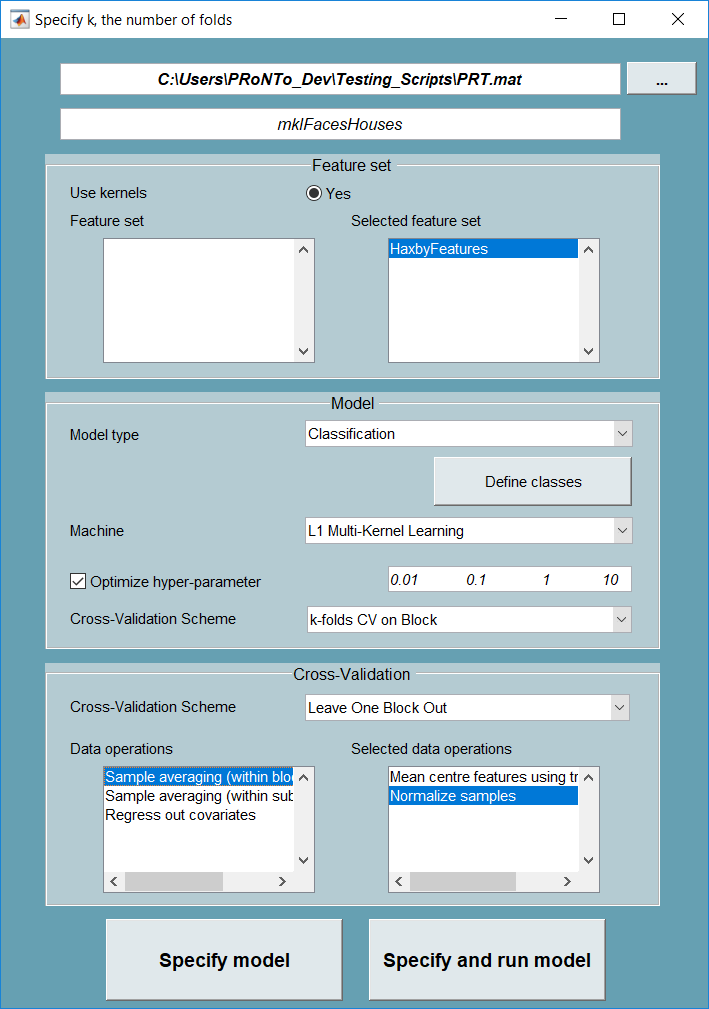
\includegraphics[width=0.5\textwidth]{images/Tutorial/v3/data_example3/data_example3_gui_model_specify_new_final.png}
	\caption{`Specify model new' GUI final configuration.}
	\label{fig:data_example3_gui_model_specify_new_final}
\end{figure}
	
	\item Click on `Specify and run model' and the model will be immediately estimated, therefore there is no need to use the `Run model' module in this case. If however you wanted to check the statistical significance of your results, you need to use the `Run model' module in order to do permutation testing. It will take a few minutes to complete.

\end{itemize}

%--------------------------------------------------------------------

\subsection{Model: Specify from}

\begin{itemize}


\item The reader is referred to Chapter \ref{sec:Block_design_fMRI_dataset} and chapter \ref{chap:ModelCrossV} for more details regarding the `Model: Specify from' module.
\end{itemize}
%--------------------------------------------------------------------

\subsection{Model: Run}

The reasons for using the `Model: Run' module and not just click `Specify and run model' in the `Model: Specify new/from' module are the following:

\begin{itemize}
\item One might want to specify one or more models now but run it/them later.
\item One might want to specify more than one models first and run them all together at once afterwards.
\item One might want to run permutation tests in order to check the statistical significance of the results. The reader is referred to Chapter \ref{sec:Block_design_fMRI_dataset} and section \ref{s:DisRes_stats} for more details.

\end{itemize}

%--------------------------------------------------------------------

\subsection{Display model (optional step)}

\begin{itemize}
\item To review the model specification, in the main PRoNTo GUI, click on `Review kernel \& CV' and after you select the `PRT.mat' file to review, a new window will open, `Review Model Specification' (Figure \ref{fig:gui_review_kernel_and_CV}) in Chapter \ref{sec:Block_design_fMRI_dataset}).

\item Select the model, `mklFacesHouses', from the list at the top and click on `Review model'; then, select one class from the list of `Class' to see which groups, subjects and conditions this class comprises, similar the one to Figure \ref{fig:gui_review_kernel_and_CV_model}) in Chapter \ref{sec:Block_design_fMRI_dataset};

\item To review the data and cross-validation matrix click on `Review CV' and a Figure similar to Figure \ref{fig:gui_review_kernel_and_CV_CV} in Chapter \ref{sec:Block_design_fMRI_dataset} will appear. For more information on what these matrices mean, please consult chapter \ref{chap:ModelCrossV}.

\item To review the kernel, click on `Show kernel' (Figure \ref{fig:data_example3_gui_review_kernel_and_CV_kernel}).

\begin{figure}[!h]
	\centering
		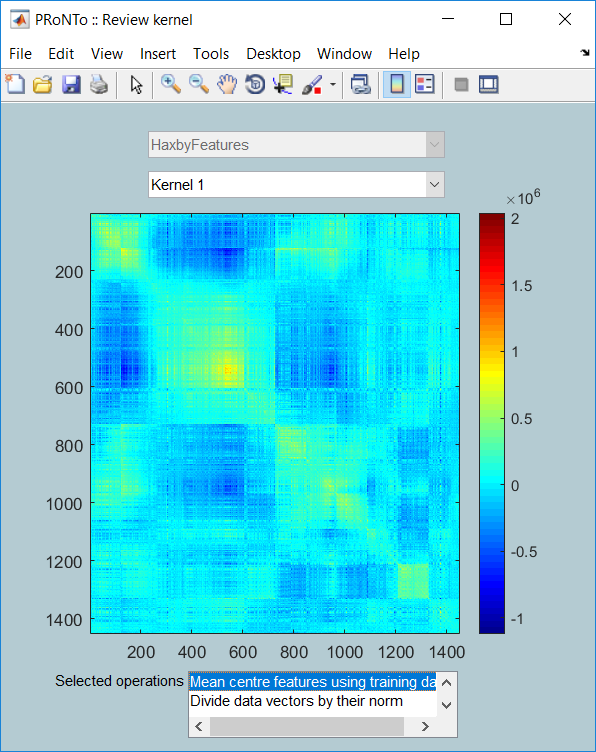
\includegraphics[scale=0.5]{images/Tutorial/v3/data_example3/data_example3_gui_review_kernel_and_CV_kernel.png}
	\caption{Kernel matrix used for classification.}
	\label{fig:data_example3_gui_review_kernel_and_CV_kernel}
\end{figure}

\end{itemize}

%----------------------------------------------------

\subsection{Display results}
\label{display_results_MKL}

\begin{itemize}
	
	\item In PRoNTo's main window, click on `Display results' and select the `PRT.mat' file. This will open the main results window. In the `Model' panel, select the model that you want to view, `mklFacesHouses', and the results through performance will be similar to the one in Figure \ref{fig:data_example3_gui_display_results};
	
	\begin{figure}[!h]
	\centering
		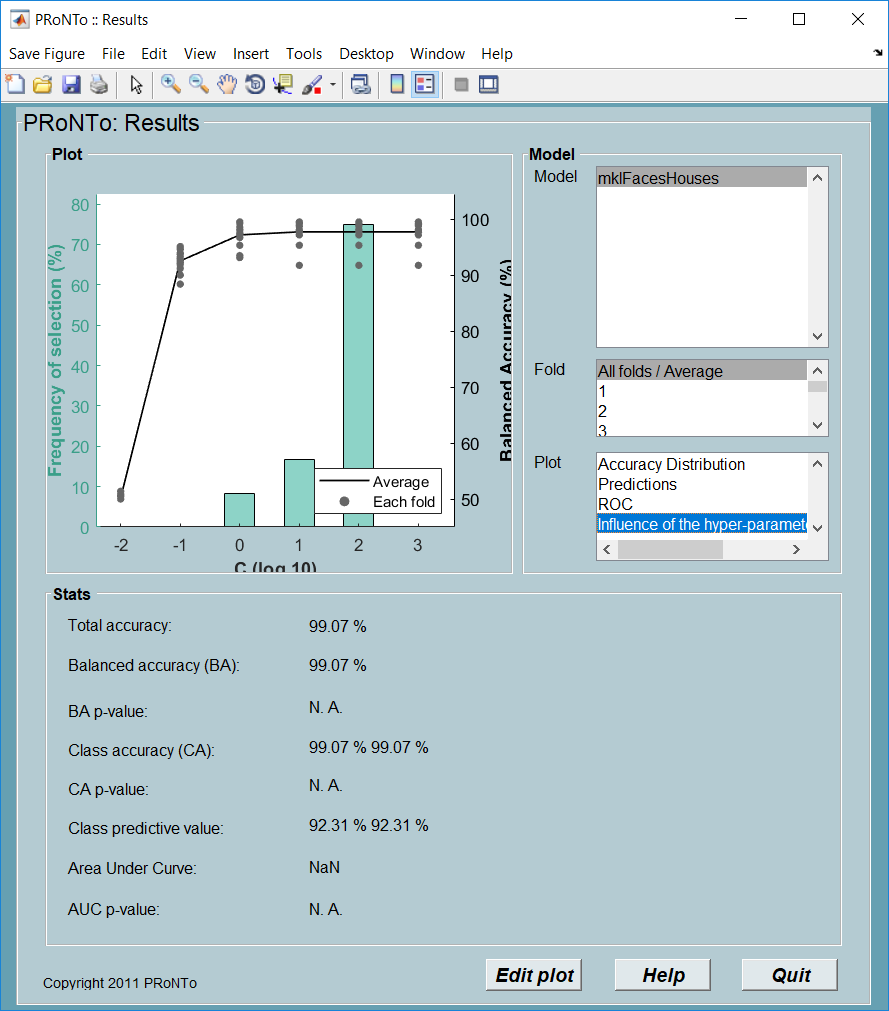
\includegraphics[width=0.5\textwidth]{images/Tutorial/v3/data_example3/data_example3_gui_display_results.png}
	\caption{`Display results' GUI.}
	\label{fig:data_example3_gui_display_results}
\end{figure}
	
	\item In the `Results' window, one can select the different plots in the `Plots' list.
	
		\item In the `Results' window, one can select specific folds in the `Fold' list and also check their performance with different plots in the `Plot' list. Please note that there is a new plot on the list, this displays information about the hyper-parameter optimization, for more information, please refer to Chapter \ref{chap:DisRes}.
	
	\item Also keep in mind that if you have not run permutation tests, all p-values would be `N.A.'.
		
\end{itemize}
	
%------------------------------------------------------------------

\subsection{Compute weights}

\begin{itemize}
\item In PRoNTo's main window, click on `Compute weights' and a new window will open, `Compute weights' (see Figure \ref{fig:gui_compute_weights} in Chapter \ref{sec:Block_design_fMRI_dataset}); 

\item Select the `PRT.mat' file;

\item Select the model from the list to `Models computed in PRT', `mklFacesHouses' model;

% \item If you previously run permutation tests and want to review and display the results, check the option `Build weight images for permutations'.

\item Check the tick box option `Compute average/kernel weight per region';

\item Click on the 'Compute weights' button. Computations will be displayed on the \matlab{} prompt.

\end{itemize}

%------------------------------------------------------------------

\subsection{Display weights}

\begin{itemize}
	
	\item In PRoNTo's main window, click on `Display weights' and select the `PRT.mat' file. This will open the primary `Display weights' window. By clicking on `Model', mklFacesHouses, an image will appear in the `Weights map' box; and to show the `Anatomical img' you have to load an anatomical image for reference. A template image can be found in the SPM's canonical folder `single\_subj\_T1'. The final result window will look similar to that shown in Figure \ref{fig:data_example3_gui_display_weights}.

    \item Since the machine used in the example was MKL with a kernel calculated for each brain region, it is possible to see the contributions of each region (i.e. the kernel's weights). The labels for the regions can be found in the same folder where the atlas is located (PRoNTo/atlas). For more information, please refer to Chapter \ref{chap:DisWeights}.

\begin{figure}[!h]
	\centering
		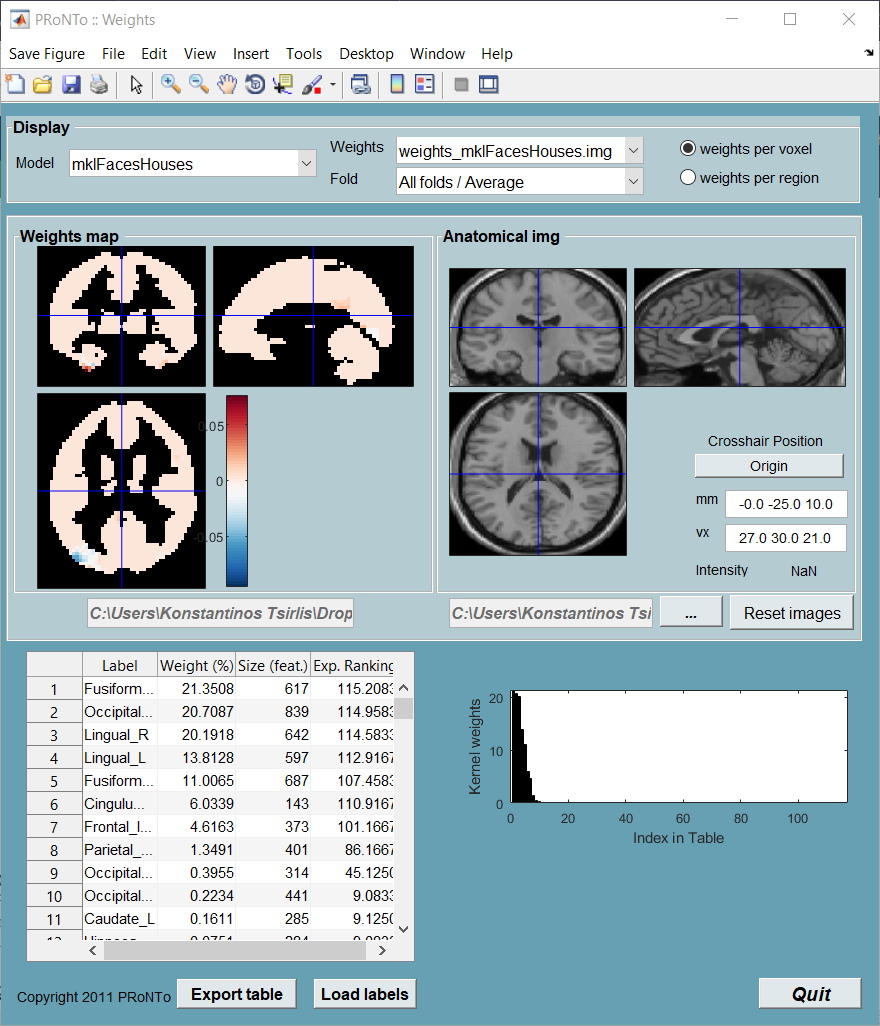
\includegraphics[width=0.5\textwidth]{images/Tutorial/v3/data_example3/data_example3_gui_display_weights.png}
	\caption{`Display weights' GUI.}
	\label{fig:data_example3_gui_display_weights}
\end{figure}
	
\end{itemize}

%=====================================================



%=====================================================

\section{Batch analysis}
\label{sec:mkl_Batch_analysis}

This tutorial will now show how to analyse the same data but using the {\tt matlabbatch} system.
\\

Once again, to analyse the data, create a new directory in which to save the results of the analysis, saved as `PRT.mat'. On the main interface of PRoNTo click on the `Batch' button to open the `{\tt matlabbatch}'. Alternatively, type `prt\_batch' in the \matlab{} prompt.

%--------------------------------------------------------------

\subsection{Data \& Design}

\begin{itemize}

	\item Click on `Data \& Design' in the PRoNTo menu and a window like the one in Figure \ref{fig:batch_data_and_design} will appear.

	\item In the `Directory' field, select a directory where the `PRT.mat' file will be saved. There are three ways of editing all fields in {\tt matlabbatch}: (i) by using the right mouse button and clicking on the current option, (ii) clicking on current button in the window or (iii) by double clicking;
	
	\item In the `Groups' field:
 	
		\begin{itemize}
		
		\item Add one group;
		
		\item In the field `Name', provide a name without spaces to that group, e.g. `G1'; 
		
		\item In the field `Select by', select the `Subjects' option and add one subject;
		
		\item Add one modality for this subject and provide a name, e.g. `fMRI'; choose the appropriate data format (here nifti); define the interscan interval of 2.5 seconds; and in the field `Files', select all the image files available in the fMRI directory of the Haxby dataset;	
		
		\item In the `Data \& Design' field, since our data are in nifti format, choose the `Load SPM.mat' option. This file is available with the Haxby dataset on PRoNTo's website\footnote{http://www.mlnl.cs.ucl.ac.uk/pronto/prtdata.html} inside the folder Haxby\_dataset/design/. The reader is referred to Chapter \ref{sec:Block_design_fMRI_dataset} in case there is no `SPM.mat' file available.


        \item The reader is referred to the tutorial of chapter \ref{sec:multimodal_face} in case the data are not in nifti format.

		\end{itemize}
	
	\item In the `Masks' field, add a new modality and provide the same modality name, `fMRI', choose the appropriate data format and finally select the `whole\_brain' mask available in the masks directory of the Haxby dataset. The name of the modality here has to be exactly the same as in `Modalities', otherwise it will not work;
	
	\item Leave the `HRF overlap' and the `HRF delay' fields as default;
	
	\item In the `Review' field, select `Yes' if you would like to review your data and design in a separate window. Otherwise, leave as it is, i.e. `No'. Keep in mind that the procedure pauses while you review the data and that you have to close the `Review' window for the procedure to continue.

\end{itemize}

The final configuration should look similar to the Figure \ref{fig:batch_data_and_design_full_final} in Chapter \ref{sec:Block_design_fMRI_dataset}.

%------------------------------------------------------------

\subsection{Feature set / Kernel}

\begin{itemize}
	\item Click on `Feature set / Kernel' option on PRoNTo's {\tt matlabbatch} menu.
	
	\item With `Load PRT.mat' field selected, click on the `Dependency' button to associate the `PRT.mat' file created in the previous `Data \& Design' step or click on the `Select files' button to browse where `PRT.mat' file was saved. The window of Figure \ref{fig:batch_feature_set_dep} in Chapter \ref{sec:Block_design_fMRI_dataset} is called to establish a dependency connection with the previous `Data \& design' module.

	\item Provide a name to the `Feature/kernel' set, e.g. `HaxbyFeatures';
	
	\item Select the `Nifti' option for a data format, add one modality and select the modality name with the `Dependency' button\footnote{Or type it in manually, `fMRI', but the name needs to be {\it exactly} the same as the one specified in the `Data \& Design' module.}(Data \& Design:Mod\#1 name);
	
		\begin{itemize}
	
	\item In the `Samples/Conditions' field , select the `All samples' option;
	
	\item In the `Voxels to include' field, select `All voxels' option;
	
	\item In the `Detrend' field, select `Polynomial detrend' option with order 1;
	
	\item In the `Scale input scans' field, select `No scaling' option.
	
	\item In the `Use atlas to build ROI specific kernels', select an atlas file AAL (named `aal\_79x91x69) available in the PRoNTo directory (PRoNTo/atlas/).
 	
	\end{itemize}
	
\end{itemize}

    Figure \ref{fig:data_example3_batch_prepare_featureSet_final} shows the final configuration of the {\tt matlabbatch} `Feature set / Kernel' module.
	

	\begin{figure}[!h]
	\centering
		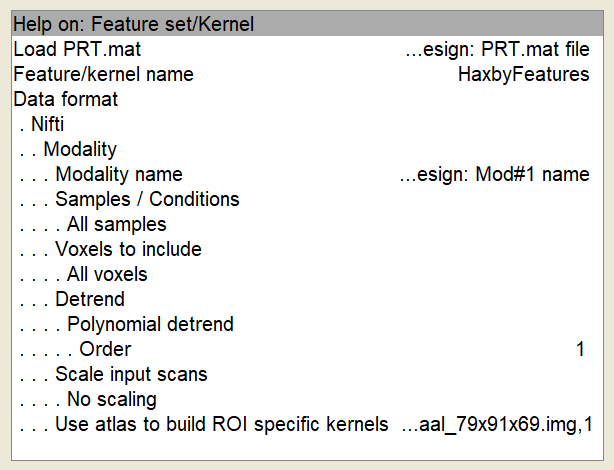
\includegraphics[width=0.5\textwidth]{images/Tutorial/v3/data_example3/data_example3_batch_prepare_featureSet_final.png}
	\caption{Final configuration of the {\tt matlabbatch} `Feature set / Kernel' module.}
	\label{fig:data_example3_batch_prepare_featureSet_final}
\end{figure}


%--------------------------------------------------------

\subsection{Model: Specify new}

\begin{itemize}

\item Click on the `Model: Specify new' option on PRoNTo's {\tt matlabbatch} menu.
	
	\item With `Load PRT.mat' field selected, click on the `Dependency' button to associate the `PRT.mat' file created in the previous `Feature set / Kernel' step or click on the `Select files' button to browse where `PRT.mat' file was saved;
	
	\item Provide a name to the model, e.g. `mklFacesHouses'; 
	
	\item In the `Feature sets' field, select the feature set name with the `Dependency' button\footnote{or write it {\it exactly} as previously defined in the `Feature set / Kernel' module (option `Feature set/Kernel: Feature/kernel name'), here `HaxbyFeatures'.};
	
	\item Select the `Classification' model type:
	
		\begin{itemize}
		
		\item Add 2 new classes;
		
		\item For Class (1) write `Faces' on the name field and add one group. Select the group name from the `Data \& Design' module (`Data \& Design:Group\#1 name') with the `Dependency' button\footnote{Or write it {\it exactly}, as previously defined in the Data \& Design' module, here `G1'}. Similarly, for Class (2) write `Houses' on the name field and add the group created in the `Data \& Design' module, `G1';	
		
		\item In the `Subjects' field, type `1' (only subject 1 is selected);
		
		\item In the `Conditions / Scans' field, select the `Specify Conditions' option and add a new condition. Provide a name for this condition, i.e. for Class (1) `Faces' and for Class (2) `Houses'. Note that this name needs to be spelled exactly as specified in the `Data \& Design' module: if you simply loaded an `SPM.mat' file for the design, you {\it must} know the names of the conditions;
		
		\end{itemize}

        \item Leave `Subsample examples based on class definition' as it is, i.e. `No'.


	\item In the `Machine' field:
	
	\begin{itemize}
	
	\item Select the `Kernel machine' and the `L1 Multi-Kernel Learning' option;	
	
	\item In the `Machine optimization and parameters' field, select the `Optimize hyper-parameter' option;
	
	\item Here we need a range of values only for the `Regularization hyper-parameter' optimization, which you can leave with the defaults (i.e. [0.01, 0.1, 1, 10, 100, 1000]);
	
	\item In the `Cross validation type for hyper-parameter optimization' (internal loop) field, select the `k-folds CV on blocks' option and on the field `k' input the value 4;
	
	\end{itemize}
	
	\item In the `Cross validation type' (external loop) field, select `Leave one block out' option;
	
	\item Leave the `Include all scans' field as it is, i.e. `No';

	\item In the `Data operations' field:
	
		\begin{itemize}
		\item  Leave the `Mean centre features' field as it is, i.e. `Yes'; 
				
		\item  Click on the `Other Operations' field and select the option `Select Operations', then add a new operation and select the `{\color{black}Normalize samples/kernels'} option;
		\end{itemize}
	
\end{itemize}

Figure \ref{fig:data_example3_batch_model_specify_new_final} shows the final configuration of the {\tt matlabbatch} `Model: Specify new' module.
	

	\begin{figure}[!h]
	\centering
		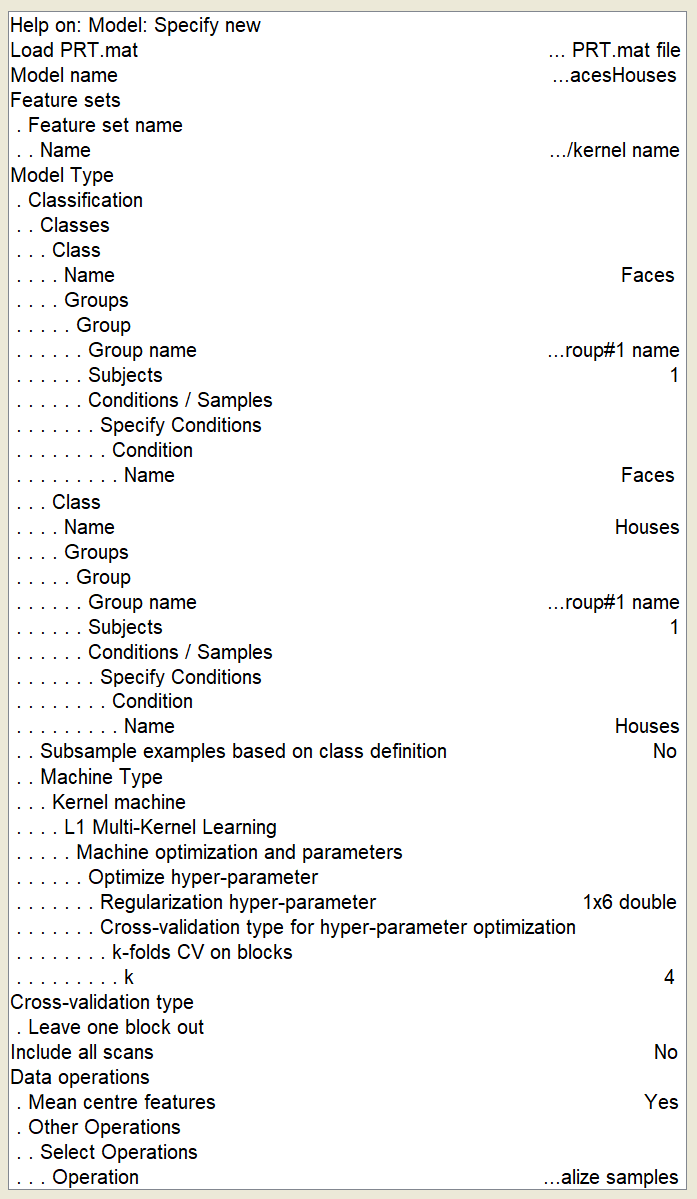
\includegraphics[width=0.47\textwidth]{images/Tutorial/v3/data_example3/data_example3_batch_model_specify_new_final.png}
	\caption{Final configuration of the {\tt matlabbatch} `Model: Specify new' module.}
	\label{fig:data_example3_batch_model_specify_new_final}
\end{figure}

%----------------------------------------------------------

\subsection{Model: Run}

\begin{itemize}

	\item Click on the `Model: Run' option on PRoNTo's {\tt matlabbatch} menu.
	
	\item  With the `Load PRT.mat' field selected, click on the `Dependency' button to associate the `PRT.mat' file created in the previous `Specify model' step;
	
	\item Select the model name from the `Model: Specify new' module with the `Dependency' button, or write it {\it exactly}, as previously defined in the `Model: Specify new' module, here `mklFacesHouses';

	\item Finally leave `Do permutation test?' as it is.
\end{itemize}

Figure \ref{fig:data_example3_batch_model_run_final} shows the final configuration of the {\tt matlabbatch} `Model: Run' module.

%-----------------------------------------------------

\subsection{Compute weights (optional step)}

\begin{itemize}

	\item Click on the `Compute weights' option on PRoNTo's {\tt matlabbatch} menu.

	\item With `Load PRT.mat' field selected, click on the `Dependency' button to associate the `PRT.mat' file created in the previous `Model: Run' step;
	
	\item Select the model name from the `Model: Specify new' module with the `Dependency' button;
	
	\item It's optional to define a name for the image; 

	\item In the `Build weight images per ROI', load the atlas that was used for building the feature set, which can be found in PRoNTo/atlas/;
	
	\item Leave the `Build weights images for permutations' field as it is, i.e. `No'; 
	

\end{itemize}

Finally, save the batch (e.g. as batch\_run\_all.m) and click on the `Run Batch' option, in the `File menu'. The batch file created can then be opened and edited for further analyses. The results will be the same as those obtained using the GUI (see Section \ref{display_results_MKL}  of this tutorial).
\\

Figure \ref{fig:data_example3_batch_compute_weights_final} shows the final configuration of the {\tt matlabbatch} `Compute weights' module.


\begin{figure}[!h]
	\centering
	\begin{minipage}[b][8.8cm][b]{0.5\textwidth}
  \centering
		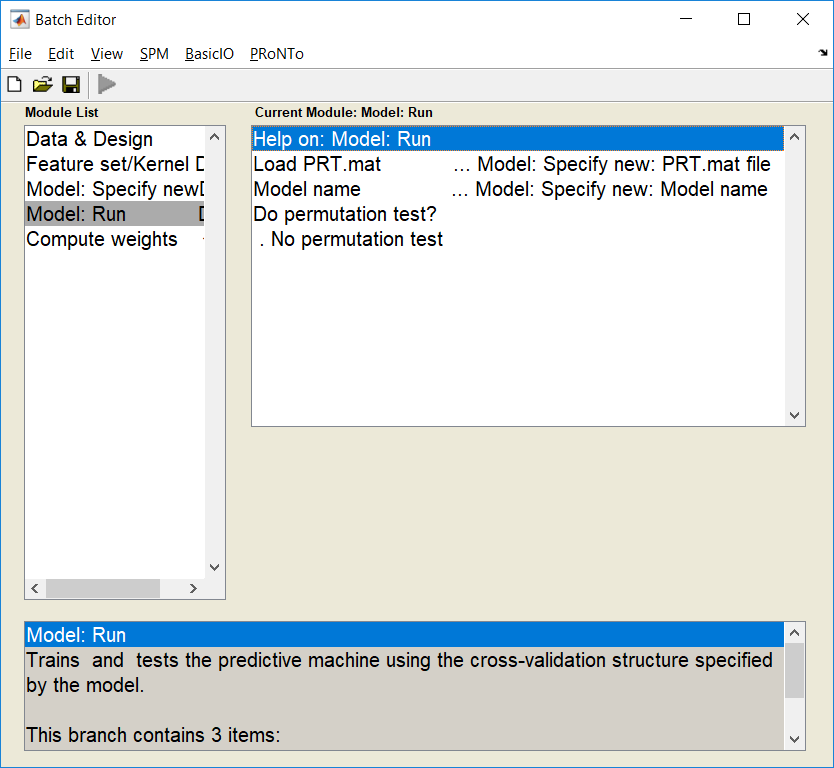
\includegraphics[scale=0.45]{images/Tutorial/v3/data_example3/data_example3_batch_model_run_final.png}
		\captionsetup{width=0.75\linewidth}
	\captionof{figure}{Final configuration of the {\tt matlabbatch} `Model: Run' module.}
	\label{fig:data_example3_batch_model_run_final}
\end{minipage}%
	\begin{minipage}[b][8.8cm][b]{0.5\textwidth}
  \centering
	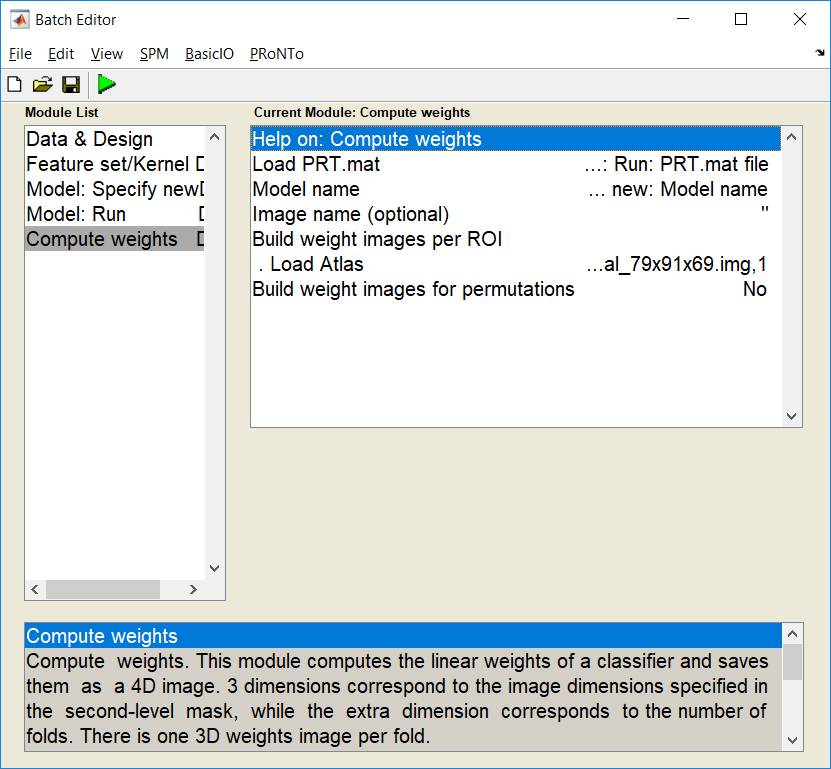
\includegraphics[scale=0.45]{images/Tutorial/v3/data_example3/data_example3_batch_compute_weights_final.png}
	\captionsetup{width=0.75\linewidth}
	\captionof{figure}{Final configuration of the {\tt matlabbatch} `Compute weights' module.}
    	\label{fig:data_example3_batch_compute_weights_final}
	\end{minipage}
\end{figure}